\chapter{نمودارهای کلاس طراحی}
({\color{red} بهنگام‌سازی شد.}) \\
در این فصل نمودارهای کلاس طراحی همراه با جزییات آن‌ها آورده شده است. به علت جلوگیری از ناخوانا شدن، از مکانیزم بسته‌بندی
\LTRfootnote{Packaging}
استفاده شده است. در هر بسته چند کلاس مرتبط به همراه ارتباطهایشان با کلاس‌های بیرونی قابل مشاهده است.
\begin{landscape}
\section{بسته پروژه}
\begin{figure}[H]
	\centering
	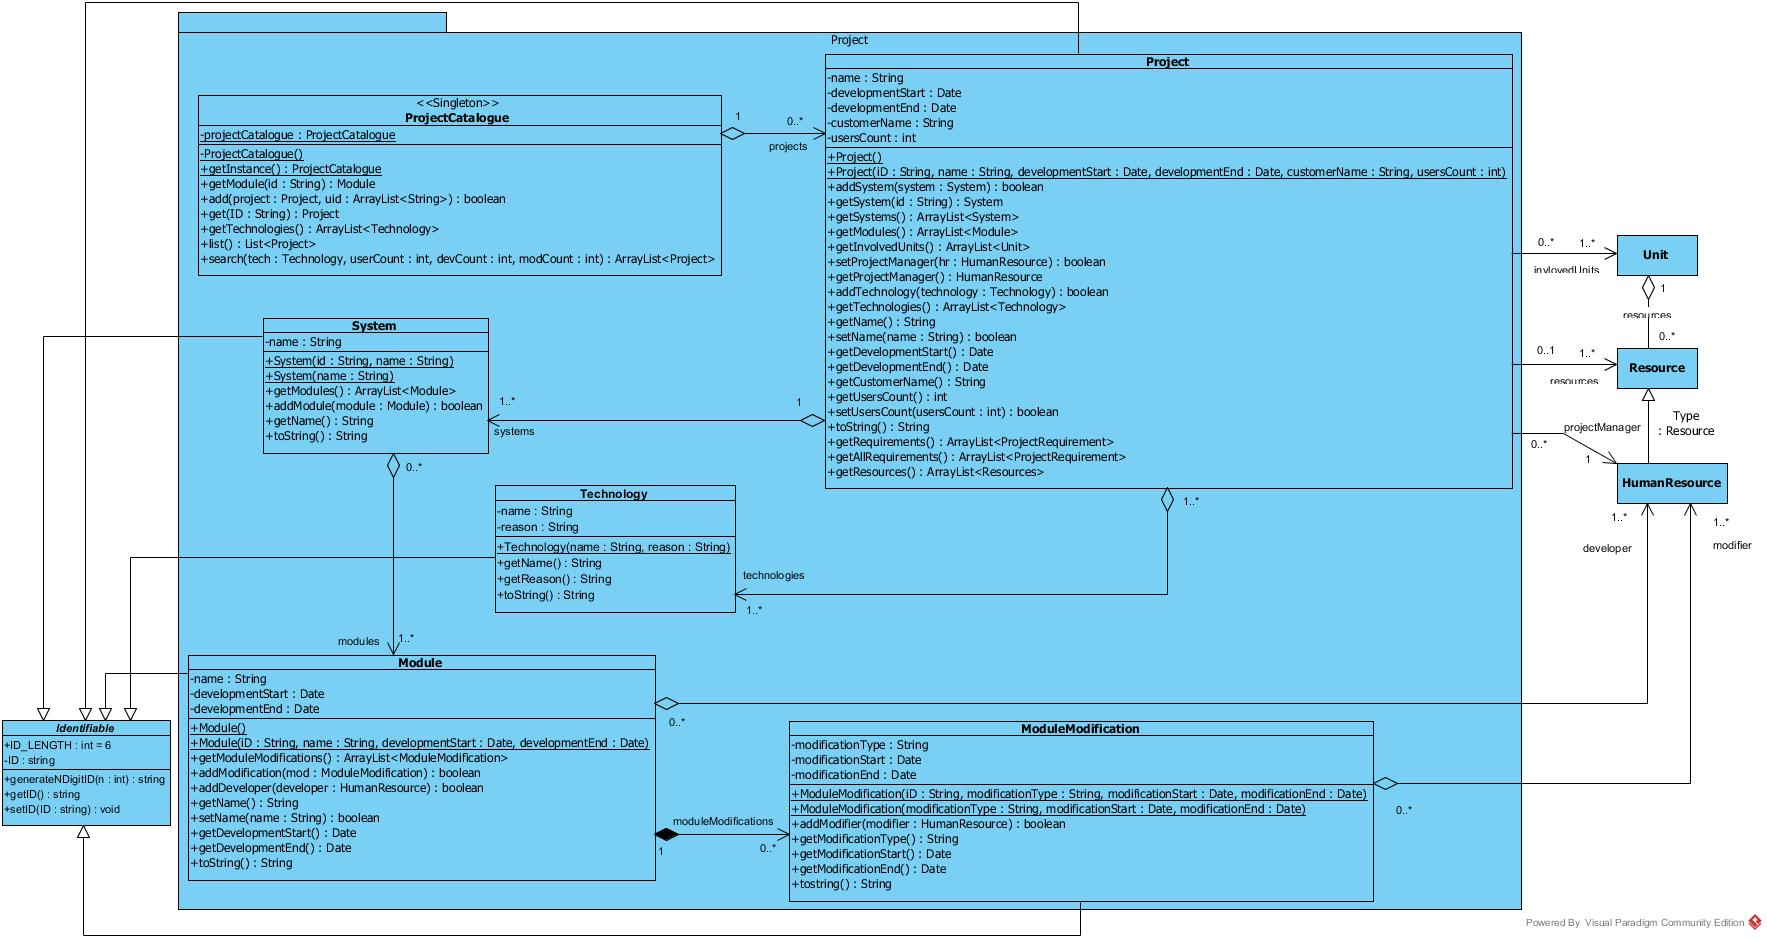
\includegraphics[scale=0.4]{img/class-design/ProjectPackage}
	\caption{بسته پروژه}
\end{figure}


\section{بسته منبع}
\begin{figure}[H]
	\centering
	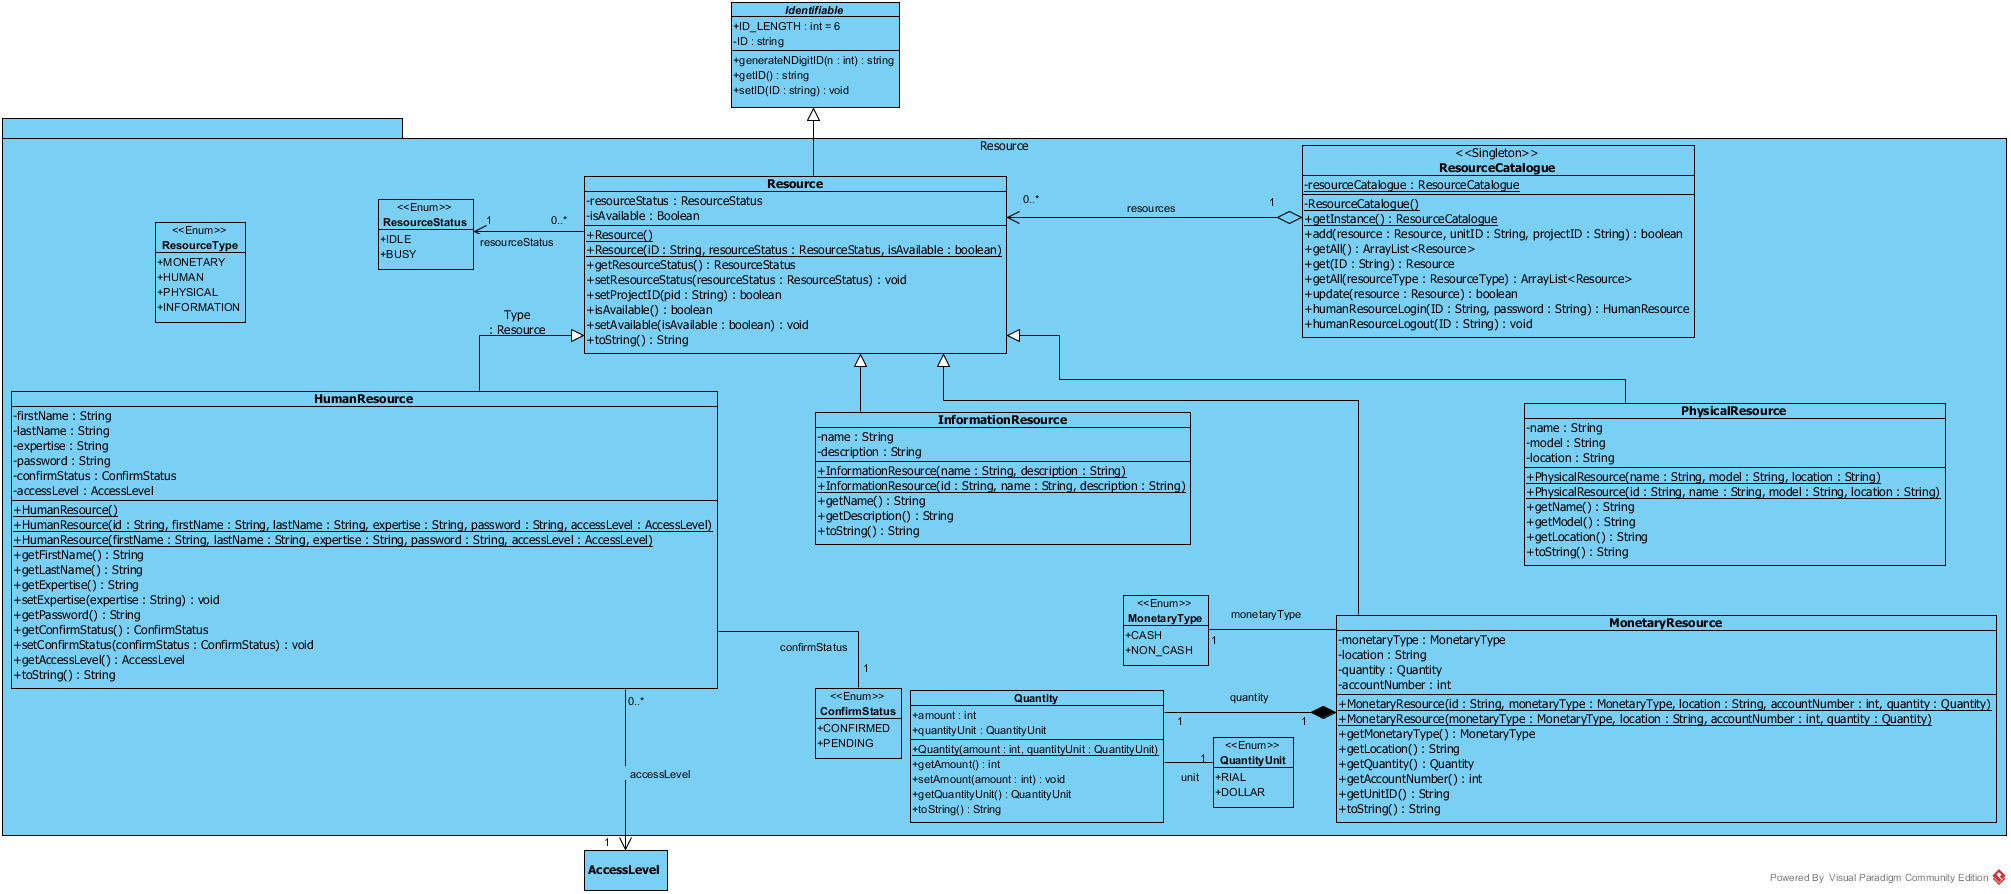
\includegraphics[scale=0.45]{img/class-design/ResourcePackage}
	\caption{بسته منیع}
\end{figure}


\section{بسته واحد}
\begin{figure}[H]
	\centering
	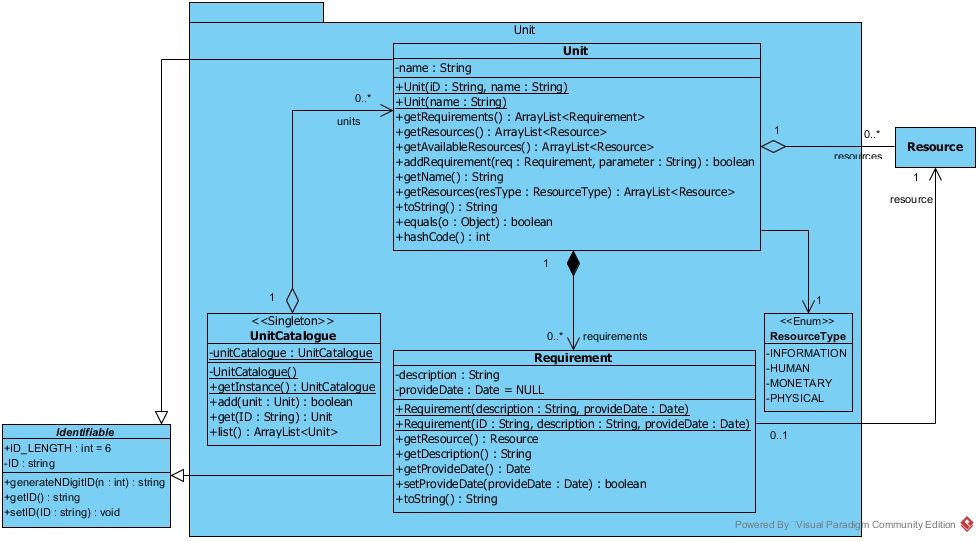
\includegraphics[scale=0.6]{img/class-design/UnitPackage}
	\caption{بسته واحد}
\end{figure}

\section{بسته گزارش}
\begin{figure}[H]
	\centering
	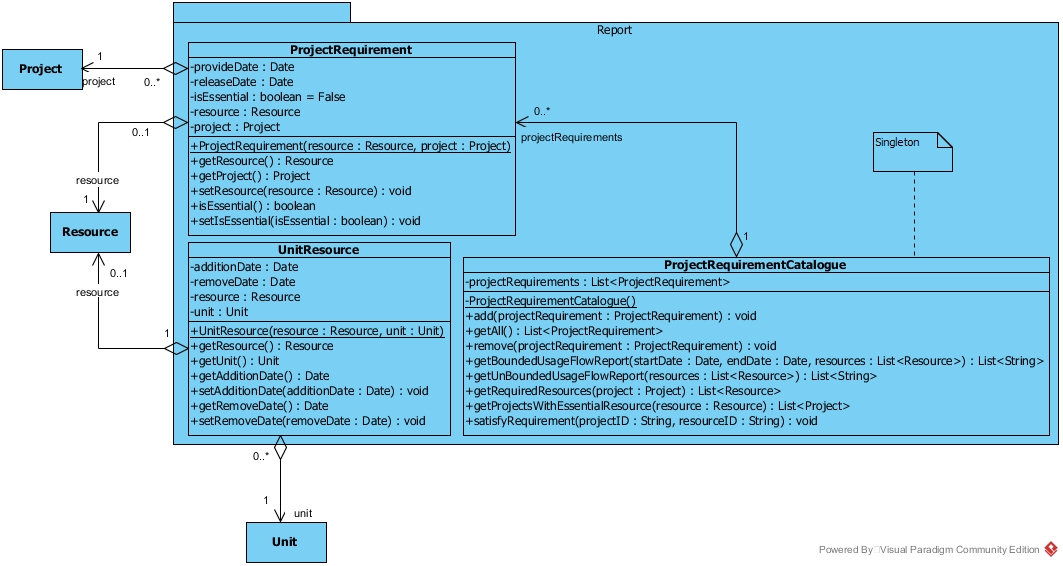
\includegraphics[scale=0.45]{img/class-design/ReportPackage}
	\caption{بسته گزارش}
\end{figure}

\section{بسته دسترسی}
\begin{figure}[H]
	\centering
	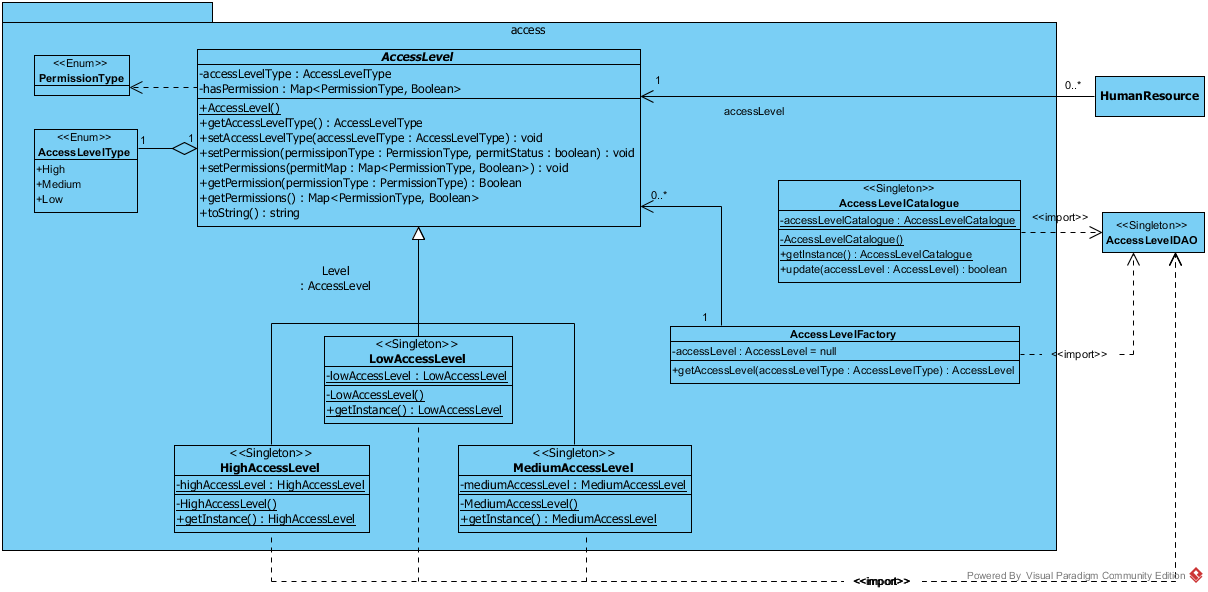
\includegraphics[scale=0.6]{img/class-design/AccessPackage}
	\caption{بسته دسترسی}
\end{figure}

\newpage
\section{بسته ارتباط لایه منطق و لایه نمایش }
کلاس‌های Facade با توجّه به کاربردشان با برخی از کلاس‌های دیگر ارتباط از نوع instantiate دارند که به منظور جلوگیری از ازدحام نمودار، تنها ا
رتباط کلاس‌های OperationFacade ، UserFacade و ProjectFacade با کلاس‌های کاتالوگ کشیده شده است.
\begin{figure}[H]
	\centering
	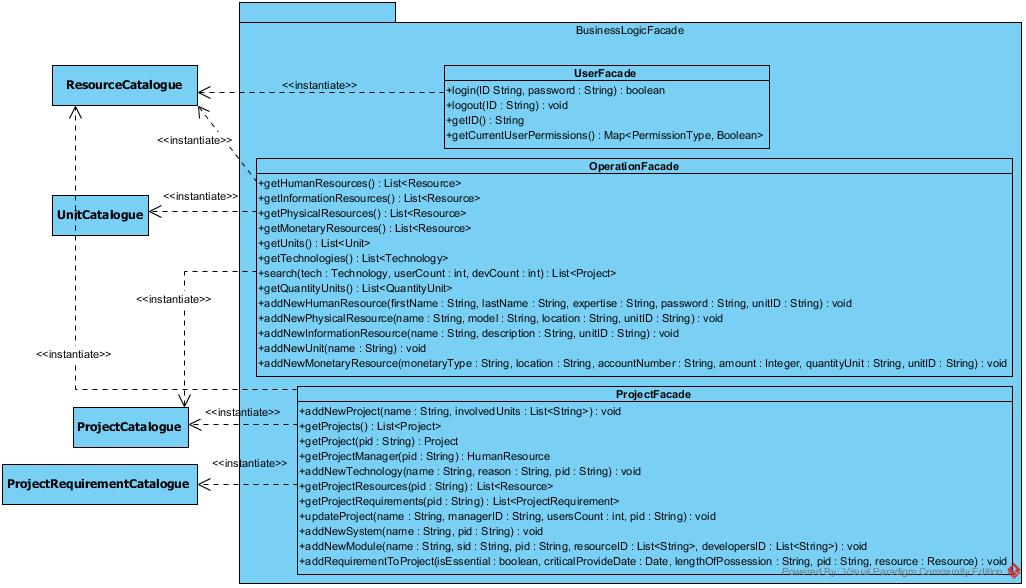
\includegraphics[scale=0.5]{img/class-design/BusinessLogicFacade}
	\caption{بسته ارتباط لایه منطق و لایه نمایش}
\end{figure}


\newpage
\section{بسته پایگاه‌داده}
از آن‌جایی که کلاس قالب
\LTRfootnote{Template}
 DAO یک واسط است، لازم است که توابع آن در همه‌ی کلاس‌هایی که به آن bind می‌شوند پیاده‌سازی شود. اما با توجه به ملاحظات مربوط به خوانایی و قرارگیری در مستند، از تکرار آن‌ها در کلاس‌های با پسوند DAO خودداری شده است.
 \\
 همچنین، کلاسی تحت نام QueryGenerator استفاده شده است که Singleton است و توابع موجود در دیگر کلاس‌های این بسته از آن استفاده کرده‌اند تا نیازی نباشد هربار پرسمان SQL به طور کامل نوشته شود. ارتباط‌های از نوع use که بین این کلاس و دیگر کلاس‌ها وجود دارد، جهت خوانایی آورده نشده است.
\begin{figure}[H]
	\centering
	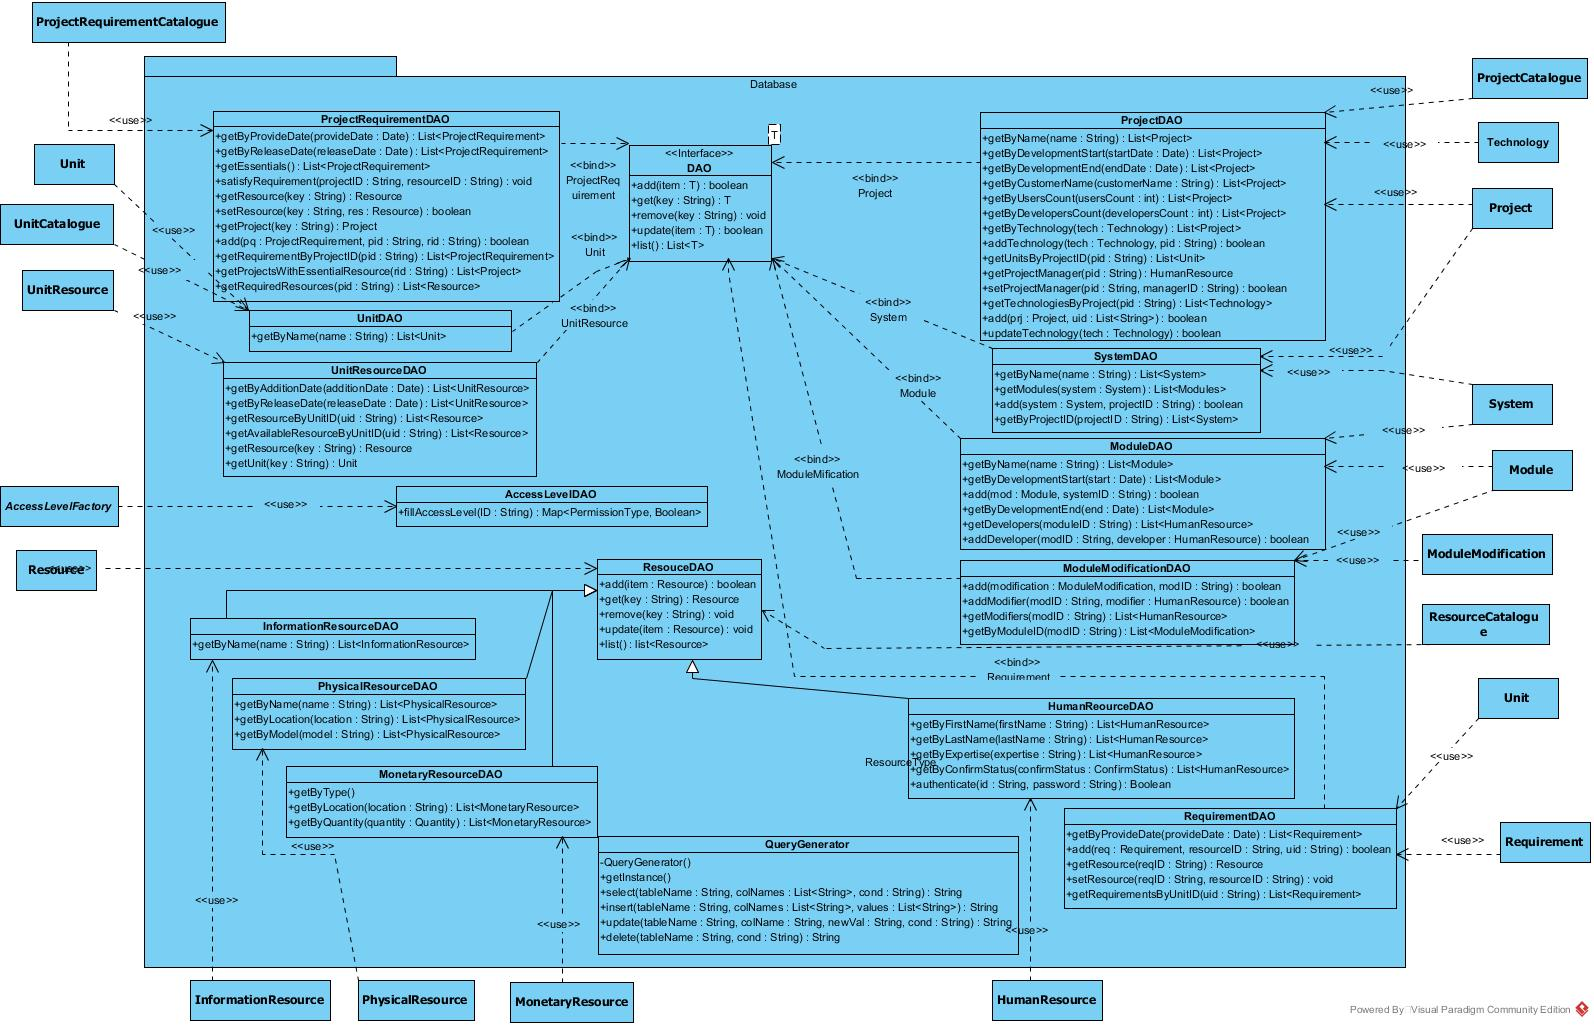
\includegraphics[scale=0.4]{img/class-design/DatabasePackage}
	\caption{بسته پایگاه‌داده}
\end{figure}
\end{landscape}


\begin{landscape}
\section{کلاس‌های واسط کاربری}
\subsection{نمای کلی کلاس‌های واسط کاربری}
همه‌ی کلاس‌های واسط کاربری ( که در واقع نمایانگر صفحات واسط کاربری هستند) از طریق واسط Visiblity می‌توانند یکدیگر را مرئی یا نامرئی کنند. در واقع همه‌ی کلاس‌های واسط کاربری از این واسط استفاده می‌کنند؛ اما برای شلوغ نشدن نمودار کلاس مربوط به آن، از آوردنش خودداری کرده‌ایم. همچنین، کلاس‌های واسط کاربری از طریق واسط دیگری (Initiator) می‌توانند یکدیگر را پیکربندی کنند. این ارتباط هم برای جلوگیری از شلوغ شدن نمودار، نمایش داده نشده است.\\
\begin{figure}[H]
	\centering
	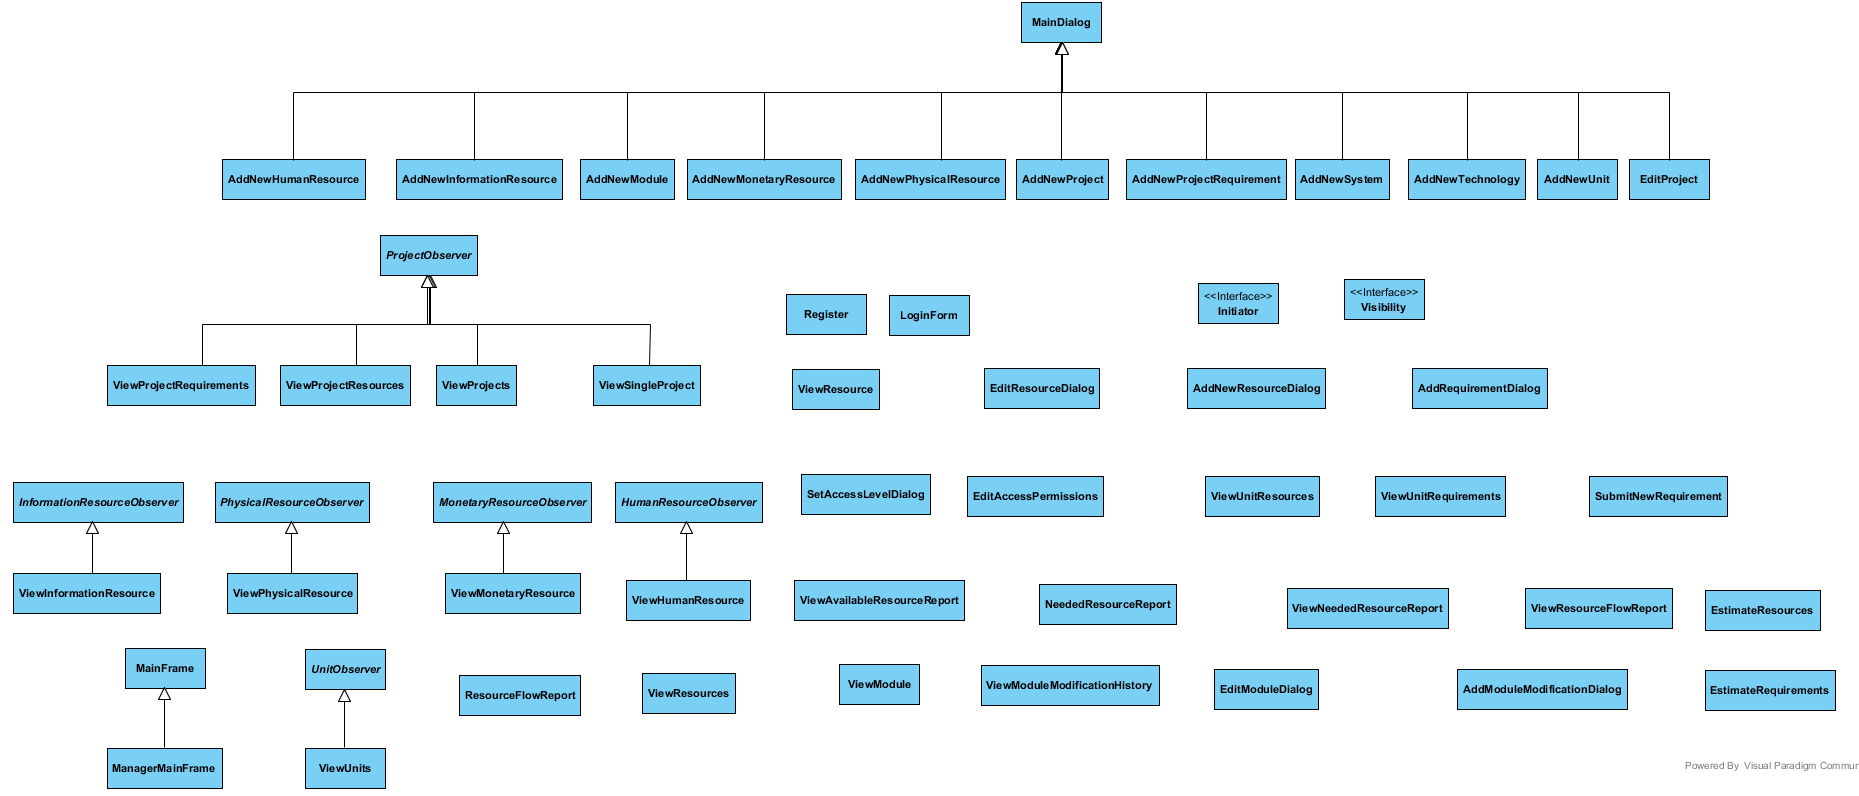
\includegraphics[scale=0.4]{img/class-design/ui/UI}
	\caption{بسته واسط کاربری}
\end{figure}
\end{landscape}

\subsection{جزییات کلاس‌های واسط کاربری}
\begin{figure}[H]
	\centering
	\begin{subfigure}[b]{0.4\textwidth}
		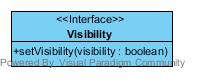
\includegraphics[width=\textwidth]{img/class-design/ui/Visibility.png}
		\caption{واسط تعیین وضعیت نمایش صفحه}
	\end{subfigure}
%	\hfill
	\begin{subfigure}[b]{0.3\textwidth}
	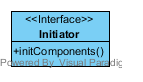
\includegraphics[width=\textwidth]{img/class-design/ui/initiator.png}
	\caption{واسط آغازگر   }			
	\end{subfigure}
	\caption{واسط‌های مورد استفاده}
\end{figure}

\begin{figure}[H]
	\centering
	\begin{subfigure}[b]{0.3\textwidth}
	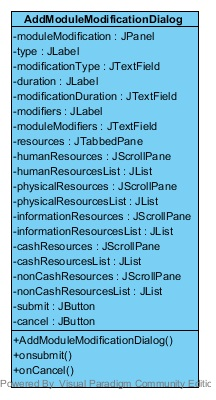
\includegraphics[width=\textwidth]{img/class-design/ui/AddModuleModificationDialog.jpg}
	\caption{کلاس ثبت تغییر ماژول}
	\end{subfigure}
	%	\hfill
	\begin{subfigure}[b]{0.3\textwidth}
	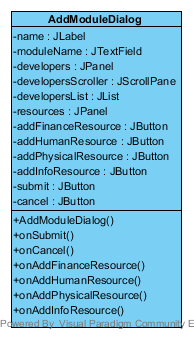
\includegraphics[width=\textwidth]{img/class-design/ui/AddModuleDialog.png}
	\caption{کلاس افزودن ماژول به سیستم}	
	\end{subfigure}
	\begin{subfigure}[b]{0.3\textwidth}
	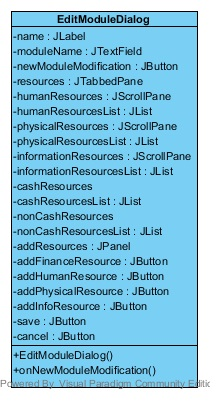
\includegraphics[width=\textwidth]{img/class-design/ui/EditModuleDialog.jpg}
	\caption{کلاس ویرایش ماژول}
	\end{subfigure}
	\caption{کلاس‌های برزش ماژول}
\end{figure}

\begin{figure}[H]
	\centering
	\begin{subfigure}[b]{0.3\textwidth}
	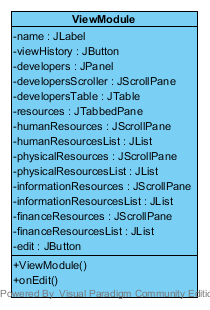
\includegraphics[width=\textwidth]{img/class-design/ui/ViewModule.png}
	\caption{کلاس مشاهده ماژول}
	\end{subfigure}
	\hfill
	\begin{subfigure}[b]{0.3\textwidth}
		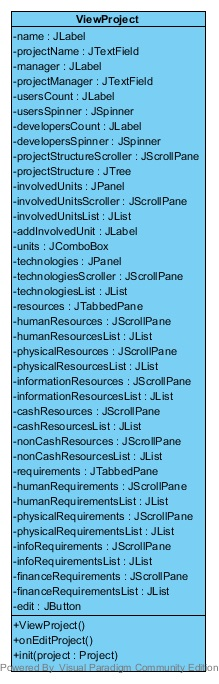
\includegraphics[width=\textwidth]{img/class-design/ui/ViewProject.jpg}
		\caption{کلاس مشاهده پروژه}
	\end{subfigure}
	\hfill
	\begin{subfigure}[b]{0.3\textwidth}
		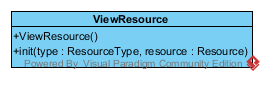
\includegraphics[width=\textwidth]{img/class-design/ui/ViewResource.png}
		\caption{کلاس مشاهده منبع}
	\end{subfigure}
	\caption{کلاس‌های مشاهده یک شئ}
\end{figure}


\begin{figure}[H]
	\centering
	\begin{subfigure}[b]{0.3\textwidth}
		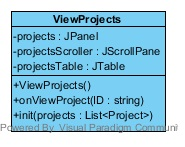
\includegraphics[width=\textwidth]{img/class-design/ui/ViewProjects.jpg}
		\caption{کلاس مشاهده پروژه‌ها}
	\end{subfigure}
	\hfill
	\begin{subfigure}[b]{0.3\textwidth}
		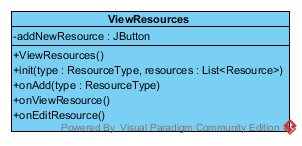
\includegraphics[width=\textwidth]{img/class-design/ui/ViewResources.jpg}
		\caption{کلاس مشاهده منابع}
	\end{subfigure}
	\hfill
	\begin{subfigure}[b]{0.3\textwidth}
		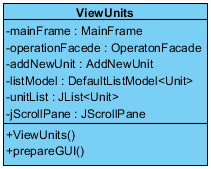
\includegraphics[width=\textwidth]{img/class-design/ui/ViewUnits.png}
		\caption{کلاس مشاهده واحدها}
	\end{subfigure}
	\hfill
	\begin{subfigure}[b]{0.3\textwidth}
		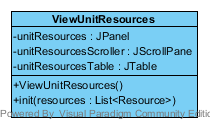
\includegraphics[width=\textwidth]{img/class-design/ui/ViewUnitResources.png}
		\caption{کلاس مشاهده منابع واحد}
	\end{subfigure}
	\hfill
	\begin{subfigure}[b]{0.3\textwidth}
		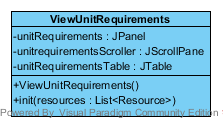
\includegraphics[width=\textwidth]{img/class-design/ui/ViewUnitRequirements.png}
		\caption{کلاس مشاهده نیازمندی‌های واحد}
	\end{subfigure}
	\hfill
	\begin{subfigure}[b]{0.3\textwidth}
		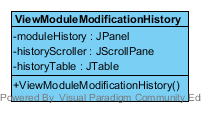
\includegraphics[width=\textwidth]{img/class-design/ui/ViewModuleModificationHistory.png}
		\caption{کلاس مشاهده تاریخچه تغییرات ماژول}
	\end{subfigure}
	\caption{کلاس‌های مشاهده چند شئ}
\end{figure}

\begin{figure}[H]
	\centering
	\begin{subfigure}[b]{0.2\textwidth}
		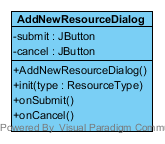
\includegraphics[width=\textwidth]{img/class-design/ui/AddNewResourceDialog.png}
		\caption{کلاس افزودن منبع جدید}
	\end{subfigure}
	\begin{subfigure}[b]{0.2\textwidth}
		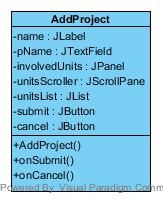
\includegraphics[width=\textwidth]{img/class-design/ui/AddProject.png}
		\caption{کلاس افزودن پروژه}
	\end{subfigure}
	\begin{subfigure}[b]{0.2\textwidth}
		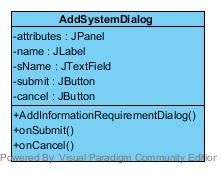
\includegraphics[width=\textwidth]{img/class-design/ui/AddSystemDialog.jpg}
		\caption{کلاس افزودن سیستم }
	\end{subfigure}
	\begin{subfigure}[b]{0.2\textwidth}
		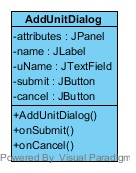
\includegraphics[width=\textwidth]{img/class-design/ui/AddUnitDialog.jpg}
		\caption{کلاس افزودن واحد }
	\end{subfigure}
	\begin{subfigure}[b]{0.2\textwidth}
		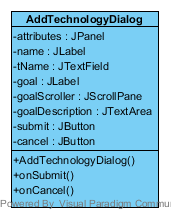
\includegraphics[width=\textwidth]{img/class-design/ui/AddTechnologyDialog.png}
		\caption{کلاس افزودن تکنولوژی به پروژه}
	\end{subfigure}
	\begin{subfigure}[b]{0.2\textwidth}
		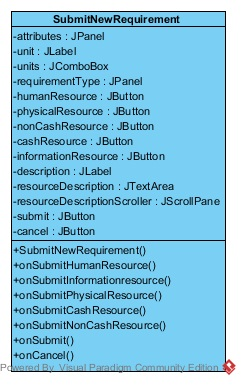
\includegraphics[width=\textwidth]{img/class-design/ui/SubmitNewRequirement.jpg}
		\caption{کلاس افزودن نیازمندی جدید}
	\end{subfigure}
	\begin{subfigure}[b]{0.2\textwidth}
		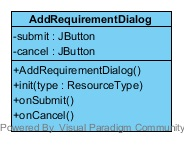
\includegraphics[width=\textwidth]{img/class-design/ui/AddRequirementDialog.jpg}
		\caption{کلاس افزودن نیازمندی}
	\end{subfigure}
	\caption{کلاس‌های افزودن یک شئ}
\end{figure}


\begin{figure}[H]
	\centering
	\begin{subfigure}[b]{0.3\textwidth}
		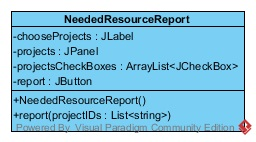
\includegraphics[width=\textwidth]{img/class-design/ui/NeededResourceReport.jpg}
		\caption{ گزارش منابع موردنیاز}
	\end{subfigure}
	\begin{subfigure}[b]{0.3\textwidth}
		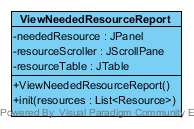
\includegraphics[width=\textwidth]{img/class-design/ui/ViewNeededResourceReport.png}
		\caption{مشاهده گزارش منابع موردنیاز}
	\end{subfigure}
	\begin{subfigure}[b]{0.3\textwidth}
		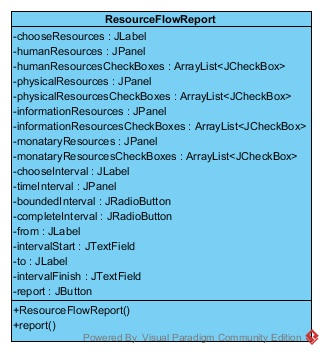
\includegraphics[width=\textwidth]{img/class-design/ui/ResourceFlowReport.jpg}
		\caption{گزارش جریان چرخشی }
	\end{subfigure}
	\begin{subfigure}[b]{0.3\textwidth}
		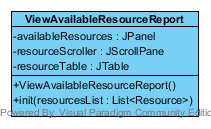
\includegraphics[width=\textwidth]{img/class-design/ui/ViewAvailableResourceReport.png}
		\caption{مشاهده گزارش منابع موجود}
	\end{subfigure}

	\begin{subfigure}[b]{0.3\textwidth}
		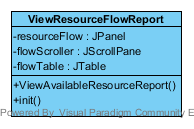
\includegraphics[width=\textwidth]{img/class-design/ui/ViewResourceFlowReport.png}
		\caption{مشاهده گزارش جریان چرخشی}
	\end{subfigure}
	\caption{کلاس‌های گزارش‌گیری}
\end{figure}

\begin{figure}[H]
	\centering
	\begin{subfigure}[b]{0.4\textwidth}
		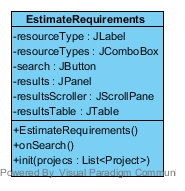
\includegraphics[width=\textwidth]{img/class-design/ui/EstimateRequirements.jpg}
		\caption{کلاس جستجو برای تخمین نیازمندی‌ها}
	\end{subfigure}
	\begin{subfigure}[b]{0.4\textwidth}
		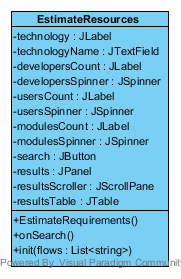
\includegraphics[width=\textwidth]{img/class-design/ui/EstimateResources.png}
		\caption{کلاس جستجو برای تخمین منابع}
	\end{subfigure}
	\caption{کلاس‌های جستجو}
\end{figure}

\begin{figure}[H]
	\centering
	\begin{subfigure}[b]{0.3\textwidth}
		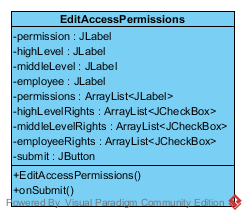
\includegraphics[width=\textwidth]{img/class-design/ui/EditAccessPermissions.png}
		\caption{کلاس ویرایش سطح دسترسی}
	\end{subfigure}
	\begin{subfigure}[b]{0.3\textwidth}
		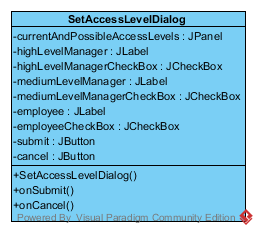
\includegraphics[width=\textwidth]{img/class-design/ui/SetAccessLevelDialog.png}
		\caption{کلاس تعیین سطح دسترسی}
	\end{subfigure}
	\caption{کلاس‌های سطح دسترسی}
\end{figure}

\begin{figure}[H]
	\centering
	\begin{subfigure}[b]{0.3\textwidth}
		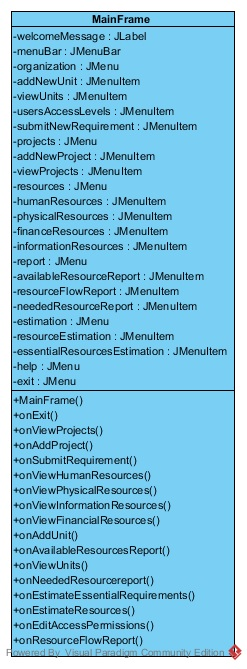
\includegraphics[width=\textwidth]{img/class-design/ui/MainFrame.jpg}
		\caption{کلاس اصلی}
	\end{subfigure}
	\begin{subfigure}[b]{0.3\textwidth}
		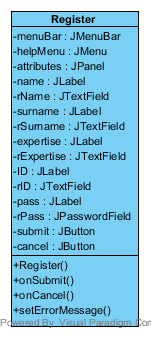
\includegraphics[width=\textwidth]{img/class-design/ui/Register.png}
		\caption{کلاس ثبت‌نام در سیستم برنامه‌ریزی}
	\end{subfigure}
	\begin{subfigure}[b]{0.3\textwidth}
		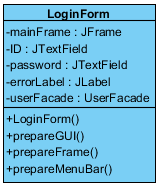
\includegraphics[width=\textwidth]{img/class-design/ui/LoginForm.png}
		\caption{کلاس ورود به سیستم برنامه‌ریزی}
	\end{subfigure}
	\begin{subfigure}[b]{0.3\textwidth}
		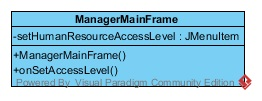
\includegraphics[width=\textwidth]{img/class-design/ui/ManagerMainFrame.jpg}
		\caption{کلاس مدیریت}
	\end{subfigure}
	\caption{کلاس‌های کاربری}
\end{figure}

\begin{figure}[H]
	\centering
	\begin{subfigure}[b]{0.3\textwidth}
		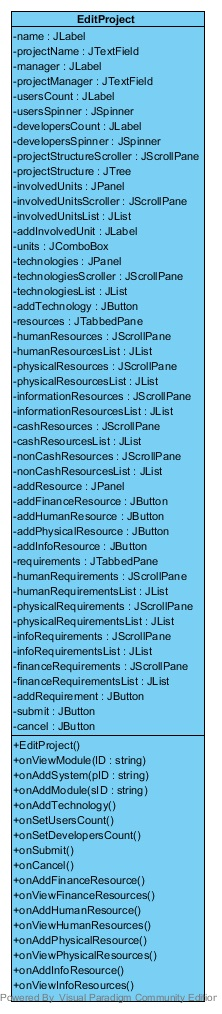
\includegraphics[width=\textwidth]{img/class-design/ui/EditProject.jpg}
		\caption{کلاس ویرایش پروژه}
	\end{subfigure}
	\begin{subfigure}[b]{0.3\textwidth}
		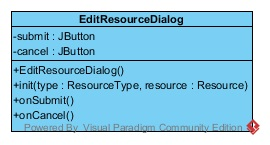
\includegraphics[width=\textwidth]{img/class-design/ui/EditResourceDialog.jpg}
		\caption{کلاس ویرایش منبع}
	\end{subfigure}
	\begin{subfigure}[b]{0.3\textwidth}
		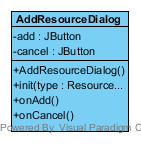
\includegraphics[width=\textwidth]{img/class-design/ui/AddResourceDialog.png}
		\caption{کلاس تخصیص منبع}
	\end{subfigure}
	\caption{کلاس‌های ویرایش شئ}
\end{figure}
